\begin{figure}[h]
    \centering
    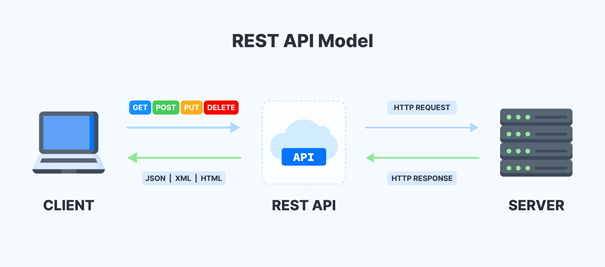
\includegraphics[scale=0.9]{sections/cloud-computing/images/rest-api.png}
    \caption{Funktionsweise von REST}
\end{figure}

Stabile und interaktive Anwendungen setzten voraus, dass Programme untereinander barrierefrei kommunizieren können. Eine API, Application Programming Interface, definiert Regeln, die diese Kommunikation erleichtert. Unter diesen Programmen kann man entweder Softwarebibliotheken, ein Betriebssystem oder einen Webserver verstehen.
Der entscheidende Vorteil von API ist, dass das anfragende Programm keinerlei Informationen über das dahinterstehende System des Antwortgebers haben muss.

\textbf{REST-API}: Einer der bekanntesten Architekturen einer API ist REST. Representational State Transfer ist ein Stil für die Entwicklung von Anwendungen, die untereinander auf irgendeine Weise vernetzt sind. Es wird oft für die Entwicklung von Web-APIs verwendet.
Wichtig zu wissen ist, dass REST zustandslos ist. In diesem Kontext bedeutet zustandslos, dass Anfragen des Clients alle notwendigen Informationen für den Server besitzen muss. Der Client kann beispielsweise nicht davon ausgehen, dass sich der Server an die vorherigen Requests des Clients erinnern kann.
REST-APIs senden im Normalfall HTTP-Anfragen wie GET, POST, PUT, etc.
